\chapter{Linear Regression with One Variable}

To establish notation for future use, we’ll use $x^{(i)}$  to denote the “input” variables (living area in this example), also called input features, and $y^{(i)}$ to denote the “output” or target variable that we are trying to predict (price). A pair ($x^{(i)}$, $y^{(i)}$) is called a training example, and the dataset that we’ll be using to learn-a list of m training examples ($x^{(i)}$, $y^{(i)}$); $i=1,...,m$ - is called a\textbf{ training set}. \\

Note that the superscript \textbf{“(i)”} in the notation is simply an index into the training set, and has nothing to do with exponentiation. We will also use X to denote the space of input values, and Y to denote the space of output values. In this example, X = Y = $\mathbb{R}$.\\

To describe the supervised learning problem slightly more formally, our goal is, given a training set, to learn a function h : X $\rightarrow$ Y so that h(x) is a “good” predictor for the corresponding value of y. For historical reasons, this function h is called a hypothesis. Seen pictorially, the process is therefore like this:

\begin{figure}[h!]
	\centering
	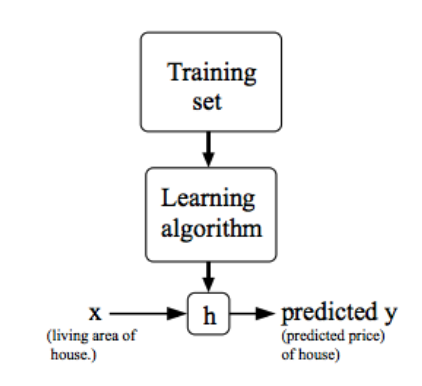
\includegraphics[width=0.5\textwidth]{fig/sl}
	\caption{Supervised learning}
\end{figure}

\section{Cost Function}

We can measure the accuracy of our hypothesis function by using a cost function. This takes an average difference (actually a fancier version of an average) of all the results of the hypothesis with inputs from x's and the actual output y's.

\begin{equation}
J(\theta_0,\theta_1)=\frac{1}{2m}\sum_{i=1}^{m}(\hat{y}_i-y_i)^2 =\frac{1}{2m}\sum_{i=1}^{m}(h_\theta(x_i)-y_i)^2
\end{equation}


Where: 

\begin{center}
$h_\theta(x_i) = \theta_0 + \theta_1\cdot x_i$
\end{center}

This function is otherwise called the "Squared error function", or "Mean squared error". The mean is halved $\left(\frac{1}{2}\right)$  as a convenience for the computation of the gradient descent, as the derivative term of the square function will cancel out the $\frac{1}{2}$ term.\\

\section{Gradient Descent}

So we have our hypothesis function and we have a way of measuring how well it fits into the data. Now we need to estimate the parameters in the hypothesis function. That's where gradient descent comes in.\\

Imagine that we graph our hypothesis function based on its fields $  \theta_0 $ and $ \theta_1 $ (actually we are graphing the cost function as a function of the parameter estimates). We are not graphing x and y itself, but the parameter range of our hypothesis function and the cost resulting from selecting a particular set of parameters.\\

We put $ \theta_0 $ on the x axis and $ \theta_1 $  on the y axis, with the cost function on the vertical z axis. The points on our graph will be the result of the cost function using our hypothesis with those specific theta parameters. The graph below depicts such a setup.\\

\begin{figure}[h!]
	\centering
	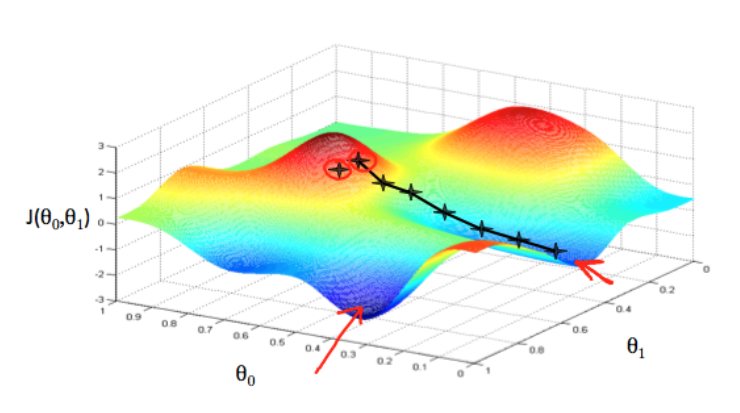
\includegraphics[width=0.8\textwidth]{fig/gradient}
	\caption{Supervised learning}
\end{figure}

\pagebreak

We will know that we have succeeded when our cost function is at the very bottom of the pits in our graph, i.e. when its value is the minimum. The red arrows show the minimum points in the graph.\\

The way we do this is by taking the derivative (the tangential line to a function) of our cost function. The slope of the tangent is the derivative at that point and it will give us a direction to move towards. We make steps down the cost function in the direction with the steepest descent. The size of each step is determined by the parameter $\alpha$, which is called the learning rate.\\

For example, the distance between each 'star' in the graph above represents a step determined by our parameter $\alpha$. A smaller $\alpha$ would result in a smaller step and a larger $\alpha$ results in a larger step. The direction in which the step is taken is determined by the partial derivative of J($ \theta_0 $,$ \theta_1 $). Depending on where one starts on the graph, one could end up at different points. The image above shows us two different starting points that end up in two different places.\\

The gradient descent algorithm is (repeat until convergence):

\begin{equation}
\theta_j := \theta_j - \alpha \frac{\partial}{\partial \theta_j} J(\theta_0, \theta_1) := \theta_j-\alpha \frac{1}{m} \sum_{i=1}^{m}\left(h_\theta(x^{(i)})-y^{(i)}\right)\cdot x^{(i)}_j
\end{equation}

Where, j=0,1 represents the feature index number.\\

\begin{center}
\textbf{Remark :} $\mathbf{ x^{(i)}_0 }$ \textbf{is ALWAYS equal 0.}\\
\end{center}

On a side note, we should adjust our parameter $ \alpha $ to ensure that the gradient descent algorithm converges in a reasonable time. Failure to converge or too much time to obtain the minimum value imply that our step size is wrong.\\

\begin{tcolorbox}[width=\textwidth,colback={lightgray},title={Correct: Simultaneous update},colbacktitle=lightgray,coltitle=blue]    
	$ temp0$ := $ \theta_0 $ - $\alpha \frac{\partial}{\partial \theta_0} J(\theta_0, \theta_1) $ \\
	$ temp1$ := $ \theta_1 $ - $\alpha \frac{\partial}{\partial \theta_1} J(\theta_0, \theta_1) $\\
	$ \theta_0 $ := $ temp0$\\
	$ \theta_1 $ := $ temp1$
\end{tcolorbox} 


